%----------------------------------------------------------------------------------------
%	ABSTRACT
%----------------------------------------------------------------------------------------

% The first character should be within \initial{}
\initial{M}{\color{teal}ε την ονομασία Unix ή μάλλον Unix-like αναφερόμαστε σε μια ολόκληρη οικογένεια λειτουργικών συστημάτων. Μερικά από αυτά είναι το linux, το Mac OS, το Solaris, το FreeBSD και άλλα. 
Τα λειτουργικά συστήματα τύπου Unix είναι σχεδιασμένα πρωταρχικά ώστε να παρέχουν περιβάλλον εργασίας για πολλαπλούς ταυτόχρονους χρήστες και συνάμα να λειτουργούν με ασφάλεια μέσα σε μεγάλα δίκτυα υπολογιστών. Είναι ακριβώς αυτή η φιλοσοφία που έχει καθιερώσει το Unix ως το κυρίαρχο λειτουργικό για servers και όχι μόνο. Δεν θα ήταν υπερβολή να ισχυριστούμε ότι το internet υπάρχει χάρη στο Unix. Πράγματι, κάθε φορά που παίρνετε κάποιο email ή ανοίγετε κάποια ιστοσελίδα, είναι σχεδόν βέβαιο ότι κάνετε χρήση κάποιου server που τρέχει Unix.
Το σύστημα αρχείων του UNIX αποτελεί μια λογική μέθοδο οργάνωσης, αποθήκευσης, αναζήτησης και διαχείρισης δεδομένων. 
Τα αρχεία είναι δομημένα σε μια ιεραρχία από καταλόγους για εύκολη αναζήτηση. H έννοια του αρχείου είναι διευρυμένη. 
Σαν αρχεία αντιμετωπίζονται όλα τα συστατικά του συστήματος, ακόμη και οι υλικές συσκευές, όπως οι εκτυπωτές και οι σκληροί δίσκοι.}

%----------------------------------------------------------------------------------------
%	ARTICLE CONTENTS
%----------------------------------------------------------------------------------------



%------------------------------------------------


\epigraphhead[10]{\epigraph{"UNIX is basically a simple operating system, but you have to be a genius to understand the simplicity."}{\textit{\href{http://en.wikipedia.org/wiki/Dennis_Ritchie}{Dennis Ritchie}}}}

\section{Εισαγωγή}

\subsection{Γιατί Unix;}

Και πάμε τώρα στο μεγάλο ερώτημα που φαντάζομαι σας ταλανίζει όλους: 
Γιατί να θέλει κάποιος να εγκαταστήσει/μάθει Unix;
Ίσως είναι λίγο νωρίς για να δοθεί απάντηση σε κάτι τέτοιο. Η επιλογή κατάλληλου λειτουργικού συστήματος είναι ζήτημα καθαρά προσωπικό και απαιτεί πολύ ψάξιμο. To σωστό ερώτημα είναι, γιατί να μην θέλει κάποιος να μάθει Unix; 

To Unix απευθύνεται κυρίως σε έμπειρους χρήστες που αναζητούν το «κάτι παραπάνω». Τα πιο mainstream λειτουργικά αποκρύπτουν πολλές
λεπτομέρειες της υλοποίησης από τον χρήστη, παρέχοντας ένα φιλικό μεν, περιορισμένο δε σύνολο λειτουργιών. Το Unix εν αντιθέσει είναι εκ
φύσεως  ανοικτό και πλήρως παραμετροποιήσιμο. Επιγραμματικά αναφέρουμε κάποια χαρακτηριστικά του: 


\begin{packed_item}
  \item \textbf{Open Source:} Τα περισσότερα Unix είναι ανοιχτού λογισμικού. O πηγαίος κώδικας (source code) διατίθεται προς όποιον το επιθυμεί, για να τον μελετήσει ή και να τον προσαρμόσει στα μέτρα του. 
  \item \textbf{Tools:} Το Unix περιέχει προεγκατεστημένη μια μεγάλη πληθώρα εργαλείων όπως compilers, βιβλιοθήκες κρυπτογραφίας, δικτυακές εφαρμογές και πανίσχυρα προγράμματα αναζήτησης που είτε δεν υπάρχουν είτε πρέπει να πληρώσετε για να τα αποκτήσετε σε άλλα λειτουργικά. Τα Unix όντας συνεχώς αναπτυσσόμενα λειτουργικά συστήματα ενσωματώνουν  τεχνολογίες που αλλού θα αργήσουν να ενεργοποιηθούν. 
  \item \textbf{Security:} Η φύση του Unix από μόνη της απαιτεί η υλοποιήση να είναι ασφαλής. Πραγματικά, είναι δύσκολο να κολλήσει κάποιο 	Unix ιό ή να αποκτήσει Spyware. Πέραν τούτου, o εντοπισμός και η διόρθωση κενών ασφαλείας είναι πολύ πιο γρήγορος και αποτελεσματικός σε λειτουργικά ανοιχτού λογισμικού. Πολλοί θεωρούν ότι το Unix σου κάνει τη ζωή δύσκολη χωρίς λόγο. Αυτό συμβαίνει διότι μερικοί προσπαθούν να δουλέψουν το Unix χωρίς να έχουν καταλάβει τη φιλοσοφία του και τη δυναμή του, κάνοντας όντως τη ζωή τους πιο δύσκολη.
\end{packed_item}

Και το πιο σημαντικό : είστε φοιτητές τμήματος Πληροφορικής, \textbf{συνεπώς δε γίνεται να μην μάθετε unix!}
Το UNIX είναι ένα λειτουργικό σύστημα για πολλούς χρήστες ο καθένας από τους οποίους μπορεί να εκτελεί ταυτόχρονα πολλές εργασίες στο σύστημα. (Multiuser-πολλοί χρήστες, Multitasking-Πολλές Διεργασίες).

Το UNIX δημιουργήθηκε το 1966 στα Bell laboratories από τον Ken Thomson σε ένα υπολογιστή DEC PDP-7 σε γλώσσα μηχανής, για εσωτερική χρήση της Bell. Ξαναγράφηκε σε C το 1973 από τον Dennis Ritchie και απέκτησε έτσι μεταφερσιμότητα (transportability). Μετά μεταφέρθηκε στα Πανεπιστήμια και έτσι απέκτησε πολλές εκδόσεις.  

Κάποια χαρακτηριστικά του unix είναι τα εξής:
\begin{packed_item}
\item Μικρά συστατικά: Το σύνολο είναι μεγαλύτερο από το άθροισμα!
\item Δυνατότητα ρύθμισης!: Όλα είναι ρυθμίσιμα, στο βαθμό που επιτρέπεται από την ασφάλεια του συστήματος!
\item Τα πάντα είναι αρχεία!
\item Το Λ.Σ. επικεντρώνεται στις διαδικασίες. Τα περισσότερα συστατικά του Unix σχεδιάστηκαν έτσι ώστε να είναι εύκολη η χρήση τους από άλλα λογισμικά. Το αποτέλεσμα είναι η υψηλή δυνατότητα «αλυσιδωτής» εκτέλεσης διεργασιών, χωρίς αλληλεπίδραση με το χρήστη.
\item Αυτοματοποίηση: Με τη χρήση κυρίως του φλοιού, βασικών εργαλείων και απλών scripting γλωσσών, όπως Perl, Python κ.α.
\item Προσαρμοστικότητα και ευελιξία
\end{packed_item}



\section{Ο φλοιός του Unix}

Ο κύριος σκοπός του φλοιού είναι να διαβάζει και να μεταφράζει τις εντολές μας καθώς μας συνδέει με το UΝΙΧ. Αυτό σημαίνει ότι δέχεται τις εντολές που δίνουμε στο τερματικό μας, ελέγχει τη σύνταξή τους, καλεί τις κατάλληλες εσωτερικές ή εξωτερικές εντολές του UΝΙΧ και επαναφέρει τον έλεγχο στον χρήστη όταν οι εντολές ολοκληρωθούν ορθά.
Κατά την ένδειξη αναμονής (Prompt), συνήθως βλέπουμε ένα χαρακτήρα από αυτούς \textbf{"\%", "\$", ή ">"}.
To prompt μπορεί να τροποποιηθεί από τον χρήστη.

Κελύφη υπάρχουν διαφόρων ειδών, και ανήκουν σε δύο κατηγορίες. Σε αυτά που είναι Bourne Shells και σε αυτά που είναι C-shells. Στο εργαστήριο θα δουλέψουμε σε Bourne Shell οπότε όλες οι εντολές θα δίνονται για αυτό \footnote{Δείτε περισσότερα στο άρθρο \href{https://www.linuxjournal.com/content/understanding-bash-elements-programming}{https://www.linuxjournal.com/content/understanding-bash-elements-programming}}. 



Τι κάνουν οι φλοιοί:
\begin{packed_enum}
  \item διαβάζουν ένα αρχείο αρχικοποίησής τους, το οποίο βρίσκεται στον κατάλογο χρήστη (home directory) και εκτελούν τις εντολές που βρίσκονται εκεί
  \item εμφανίζουν το prompt και περιμένουν εντολές από τον χρήστη
  \item περιμένουν εντολή/χαρακτήρες τερματισμού τους
\end{packed_enum}

\begin{figure}[h]
\centering
\scalebox{0.7}{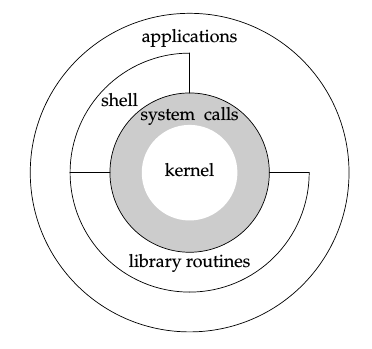
\includegraphics{images/unix_architecture.png}}
\caption{Η αρχιτεκτονική του Unix \cite{Stevens:2013}}
\end{figure} 


\begin{center}
\begin{table}[h]
\begin{tabular}{ l | l }
  / & Ο κατάλογος "κορυφής" ή ρίζα (root)  \\
  /bin & Περιέχει μεγάλο μέρος των εντολών  \\
  /dev & Ο κατάλογος των περιφερειακών  \\
  /lib & Περιέχει βιβλιοθήκες προγραμμάτων \\
  /tmp & Περιέχει προσωρινά αρχεία \\
  /usr & Περιέχει αρχεία υποστήριξης \\
  /etc & Εντολές του super-user, \\
      &	αρχεία UNIX, config files \\
  /home& Οι κατάλογοι των χρηστών \\
\end{tabular}  
\caption{Το σύστημα αρχείων του Unix}
\end{table}

\end{center}

Υπάρχουν πολλοί φλοιοί, οι οποίοι συνοψίζονται στην εικόνα \ref{os_shells}.


\begin{tcolorbox}[frogbox, title=zsh]
	Αν ενδιαφέρεστε για ένα πιο «φρέσκο» και «όμορφο» φλοιό, μπορείτε να δείτε τον zsh. Επίσης μπορείτε να εγκαταστήσετε το πακέτο \href{https://github.com/robbyrussell/oh-my-zsh}{oh-my-zsh} το οποίο έχει αρκετά έτοιμα themes.
\end{tcolorbox}

\begin{figure*}[h]
	\centering
	\scalebox{0.7}{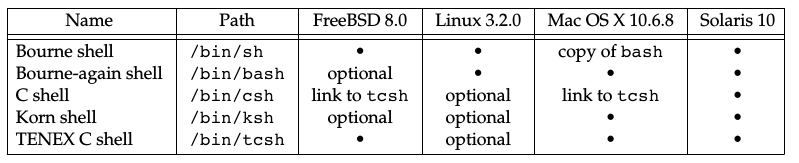
\includegraphics{images/shells_per_os.png}}
	\caption{Συνηθισμένοι φλοιοί του UNIX}
	\label{os_shells}
\end{figure*} 

\subsection{Απομακρυσμένη σύνδεση}

Ο Secure Shell ή SSH είναι ένα πρωτόκολλο δικτύου που επιτρέπει τη μεταφορά δεδομένων χρησιμοποιώντας ένα ασφαλές κανάλι μεταξύ δύο δικτυακών συσκευών \footnote{\href{https://support.suso.com/supki/SSH\_Tutorial\_for\_Linux}{SSH tutorial}}. 
	Χρησιμοποιείται κυρίως στα unix λειτουργικά συστήματα και προστατεύει ευαίσθητα δεδομένα όπως passwords. Δοκιμάστε να συνδεθείτε με ssh σε έναν server μας, ως εξής:
\begin{lstlisting}
ssh user@server
\end{lstlisting}
για παράδειγμα 
\begin{lstlisting}
ssh it21701@10.100.51.113
\end{lstlisting}
%Εκεί θα διαπιστώσετε τι σημαίνει ότι πολλοί χρήστες δουλεύουν ταυτόχρονα στον ίδιο υπολογιστή!

\section{Εντολές}

Μορφή εντολής UNIX
\begin{lstlisting}
[prompt]$ <command> <flags> <args>
\end{lstlisting}


\begin{center}
\begin{packed_item}

\item Η πρώτη λέξη είναι η εντολή 
\item Το υπόλοιπο τμήμα, αν υπάρχει, είναι επιλογές (options) και ορίσματα (arguments)‏
\item Οι εντολές είναι case sensitive (διαφορά μεταξύ κεφαλαίων και μικρών) και γράφονται με μικρά γράμματα
\item Μια εντολή μπορεί να έχει ή να μην έχει επιλογές ή ορίσματα \textbf{(π.χ. date , ls -l)}
\item Τα ορίσματα είναι συνήθως αρχεία και κατάλογοι
\item επιλογές: 
\begin{itemize}
\item Μεμονωμένα γράμματα 
\item Προηγείται μια παύλα “-”
\item Συνδυασμός ή διαχωρισμός (π.χ. -al   =   -a -l)‏
\item Προηγούνται άλλων ορισμάτων
\end{itemize}	
\item Πρέπει να υπάρχουν κενά μεταξύ των εντολών, των επιλογών και των ορισμάτων
%\item Πολλαπλές εντολές διαχωρίζονται με “;” και εκτελούνται σειριακά.
%\item Χαρακτήρες ελέγχου: Ctrl-c, Ctrl-h, Ctrl-z, …
\item On-line βοήθεια (man pages)‏
\end{packed_item}
\end{center}

Πιο συγκεκριμένα εκτελέστε τις παρακάτω εντολές που εμφανίζονται στον πίνακα \ref{tab:cmd}, και δείτε τη σύνταξή τους με τα ορίσματά τους
με την εντολή man\\

\begin{mybox}{Το manual των εντολών}
Κάθε εντολή έχει συνήθως και ένα manual που τη συνοδεύει. Πάντα να συμβουλεύεστε το man γιατί από σύστημα σε σύστημα διαφοροποιούνται. \\

\textbf{[prompt]\$ man <command>}
	
\end{mybox}

\begin{center}
\begin{table*}[h]
%\footnotesize
\begin{tabular}{ r | l }
who  & ποιοι χρήστες επικοινωνούν με το σύστημα τώρα  \\
date & μας επιστρέφει την ημερομηνία και την ώρα  \\
calc & μας επιστρέφει το ημερολόγιο του τρέχοντος μήνα \\
man όνομα-εντολής & ενημέρωση για μια εντολή \\  
pwd  & εμφανίζει τον τρέχοντα κατάλογο \\
ls & λίστα αρχείων \\
cd   & αλλάζει κατάλογο \\  
mkdir & δημιουργεί κατάλογο \\
rmdir & διαγράφει κατάλογο \\  
%mail & επικοινωνία μεταξύ των χρηστών του συστήματος  \\
cat όνομα-αρχείου & μας δείχνει το περιεχόμενο των αρχείων \\
mv & «μετακινεί» ένα όνομα αρχείου σε ένα άλλο \\
cp & αντιγράφει ένα αρχείο σε ένα άλλο \\
rm & διαγράφει αρχεία \\
\end{tabular}  
\caption{εντολές του unix} 
\label{tab:cmd}          
\end{table*}
\end{center}

%\begin{figure}
%\centering
 %\scalebox{0.2}{\includegraphics{unix-tree.eps}}
%\resizebox{\linewidth}{!}{\includegraphics{unix-tree.eps}}
%\caption{Το γενεαλογικό δέντρο του unix}
%\end{figure} 

\subsection{Μερικές παρατηρήσεις}


\begin{packed_item}
  \item Στο κέλυφος, συνήθως όταν το prompt έχει το \# σημαίνει ότι είμαστε χρήστης με επιπλέον δικαιώματα, αλλιώς στο prompt μας έχει \$.
  \item Με το σύμβολο \textbf{.} αναφερόμαστε στον τρέχοντα κατάλογο, με το σύμβολο \textbf{..} αναφερόμαστε στον γονικό κατάλογο του τρέχοντος, ενώ με το σύμβολο \space \textbf{\textasciitilde} \space αναφερόμαστε στον home directory μας \footnote{στον φλοιό bash - Bourne Again SHell }. 
  \item Προσοχή στα κεφαλαία και τα πεζά γράμματα!   
  \item Ο απλός χρήστης δεν μπορεί να κάνει shutdown τον υπολογιστή.
  \item Όταν δουλεύετε στο φλοιό δεν υπάρχει κάδος ανακύκλωσης. Ό,τι σβήσατε το χάσατε.                    
\end{packed_item}


\subsection{Τι δεν πρέπει να κάνουμε στο unix}

Δεν πρέπει ποτέ να κλείνετε το ρεύμα (ή να πατάτε το κουμπί για να κλείσει) σε ένα υπολογιστή που τρέχει unix, εκτός αν γνωρίζετε πολύ καλά τι κάνετε. Ένα unix σύστημα δεν είναι το ίδιο με ένα σύστημα που τρέχει windows. Ακόμη και αν εσείς δεν κάνετε κάτι στον υπολογιστή σας, ο υπολογιστής εκτελεί κάποιες διεργασίες στο παρασκήνιο. Αν κλείσετε το ρεύμα, μπορεί να διακόψετε το σύστημα την ώρα που γράφει στο δίσκο και να καταστρέψετε το δίσκο σας. Πρέπει επίσης να θυμάστε ότι μπορεί την ίδια στιγμή να είναι συνδεδεμένοι στο σύστημά σας κι άλλοι χρήστες, τους οποίους εσείς δεν βλέπετε: μπορεί να έχουν συνδεθεί μέσω δικτύου. Αν κλείσετε τον υπολογιστή, μπορεί να καταστρέψετε τη δουλειά τους. 


\begin{comment}
\section*{Τι θα δούμε στη συνέχεια}
\begin{packed_item}
 \item \textbf{Εισαγωγή στο UNIX}
\begin{packed_item}
 \item Διαχείριση αρχείων - Καταλόγων
 \item Ανακατεύθυνση εισόδου - εξόδου
 \item Διοχετεύσεις (pipes)
 \item Κανονικές εκφράσεις
 \item Διαχείριση διεργασιών
 \item Χρήστες, ομάδες και δικαιώματα
 \item Μεταβλητές
 \item shell scripts
 \item Δομές εκτέλεσης υπό συνθήκη
\end{packed_item}
\item \textbf{Προγραμματισμός Λειτουργιών του UNIX σε C}
\begin{packed_item}
 \item Χειρισμός Λαθών
 \item Διαχείριση Διεργασιών
 \item Κλήσεις συστήματος
 \item Αποστολή / Παραλαβή Σημάτων 
 \item Είσοδος / Έξοδος χαμηλού επιπέδου
 \item Επικοινωνία μεταξύ διεργασιών
 \item Νήματα
\end{packed_item}
\end{packed_item} 
\end{comment}

\subsection{Διαχείριση αρχείων - Καταλόγων}

\subsubsection{Απόλυτο και σχετικό μονοπάτι}
Για να αλλάξουμε κατάλογο χρησιμοποιούμε την \texttt{cd} (change directory). 
'Οταν βρισκόμαστε σε κάποιον κατάλογο και θέλουμε να μεταβούμε σε κάποιον άλλο, μπορούμε να το κάνουμε με δύο τρόπους:
\begin{packed_item}
  \item Δίνοντας το απόλυτο μονοπάτι, ξεκινώντας από τη ρίζα \textbf{/}. Για παράδειγμα αν είμαστε στον \textbf{/home/bill} και θέλω να πάω 	στον \textbf{/home/bill/Desktop} θα δώσω\textbf{ cd /home/bill/Desktop}.
  \item Δίνοντας το σχετικό μονοπάτι από τη θέση που βρισκόμαστε. Για παράδειγμα αν είμαστε στον \textbf{/home/bill} και θέλω να πάω στον \textbf{/home/bill/Desktop} θα δώσω \textbf{cd Desktop}.
\end{packed_item}

Πριν είχαμε εκτελέσει την εντολή \texttt{ls} για να βλέπουμε τα περιεχόμενα ενός καταλόγου (μαζί με παραμέτρους). Τώρα θα δούμε πως δημιουργούμε αρχεία και καταλόγους.

\subsubsection{Διαχείριση καταλόγων}
Η εντολή \texttt{mkdir} δημιουργεί έναν κατάλογο (συνήθως στον κατάλογο που είμαστε, εκτός αν ορίσουμε το απόλυτο μονοπάτι και
δημιουργήσουμε κάπου αλλού έναν κατάλογο).

Για να διαγράψουμε έναν άδειο κατάλογο, χρησιμοποιούμε την εντολή \texttt{rmdir}. 

\subsubsection{ls}
Η εντολή με την οποία φαίνονται τα περιεχόμενα του καταλόγου είναι η εντολή ls.
Αν δώσουμε με την ls την παράμετρο –a τότε μπορούμε να δούμε και τα κρυφά αρχεία. Κρυφά είναι τα αρχεία των οποίων τα ονόματα τους αρχίζουν από τελεία όπως πχ το .profile για το κέλυφος bourne. Άμα με την ls δώσουμε την παράμετρο –l τότε μας εμφανίζονται λεπτομέρειες για τα αρχεία του καταλόγου. Φυσικά μπορούμε να δώσουμε και τις δύο παραμέτρους και να γράψουμε ls –al οπότε θα έχουμε και λεπτομέρειες και την
εμφάνιση των κρυφών αρχείων. Με αυτήν την ευκαιρία μπορούμε να εξηγήσουμε με
λεπτομέρεια τι βλέπουμε στην οθόνη όταν εκτελέσουμε την εντολή ls –al.
Η πρώτη στήλη αφορά το είδος των αρχείων και τα δικαιώματα που έχουν οι χρήστες
σε αυτά. Στην δεύτερη στήλη φαίνονται οι σκληροί σύνδεσμοι (hard links) του κάθε
αρχείου ή αλλιώς με πόσα ονόματα παρουσιάζεται αυτό το αρχείο στο σύστημα
αρχείων (filesystem). Στην τρίτη στήλη είναι ο χρήστης που είναι ο ιδιοκτήτης του
αρχείου, ενώ στην τέταρτη είναι η ομάδα χρηστών στην οποία ανήκει το
συγκεκριμένο αρχείο. Η πέμπτη στήλη έχει το μέγεθος του αρχείου σε blocks. Οι
επόμενες τρεις στήλες έχουν με την σειρά τον μήνα, την ημερομηνία και την ώρα
δημιουργίας του αρχείου, ενώ η τελευταία στήλη έχει το όνομα του αρχείου.

\subsubsection{Εντολές cat, more, less}

Οι εντολές οι οποίες δείχνουν τα περιεχόμενα ενός αρχείου είναι οι cat, more, less. Η
cat δείχνει τα περιεχόμενα όλα μαζί. Αυτό σημαίνει ότι όταν το αρχείο είναι αρκετά
μεγάλο και δεν φτάνει μια οθόνη για να δούμε τα περιεχόμενα του με την cat τα
περιεχόμενα θα «τρέξουν» από μπροστά μας και δεν θα προλάβουμε να δούμε τίποτα.
Σε τέτοια περίπτωση θα πρέπει να χρησιμοποιήσουμε την more ή την less. Αυτές
έχουν το πλεονέχτημα ότι δείχνουν τα περιεχόμενα οθόνη-οθόνη οπότε έχουμε την
ευχέρεια να τα μελετήσουμε με την ησυχία μας. Για να πάμε στην επόμενη οθόνη
πατάμε το πλήκτρο <space> ενώ το πλήκτρο <enter> μας πάει στην επόμενη σειρά.
Επίσης είναι δυνατή η δημιουργία αρχείου κειμένου με την εντολή cat. Γράφοντας
cat > filename η εντολή περιμένει είσοδο από το πληκτρολόγιο και δίνει έξοδο στο
αρχείο filename. Ο τερματισμός εισόδου δεδομένων γίνεται με <Ctrl-D>.

\subsection{Μεταχαρακτήρες}

Oι µεταχαρακτήρες wildcard ή µπαλαντέρ µπαίνουν στις εντολές για να αντικαταστήσουν ονόµατα ή µέρος τoυ ονόµατος αρχείων και καταλόγων.
Υπάρχουν τριών ειδών μεταχαρακτήρες (wildcards):

\begin{packed_item}
  \item * : αντικαθιστά από κανέναν έως όλους τους χαρακτήρες ενός ονόµατος. Παράδειγμα:
        \begin{packed_item}
            \item ls * λίστα με όλα (αρχεία και κατάλογοι)
            \item ls *.* λίστα με εκείνα που στο όνομά τους υπάρχει τελεία
            \end{packed_item}
  \item ? : αντικαθιστά ένα ακριβώς χαρακτήρα ενός ονόματος
        \begin{packed_item}
            \item ls ? λίστα με εκείνα που το όνομά τους είναι ένας χαρακτήρας
            \item ls lab? λίστα με εκείνα που το όνομά τους ξεκινά με lab και μετά ακολουθεί ένας χαρακτήρας πχ. lab1,lab2,lab3,labx.
            \end{packed_item}
  \item $[c]$ : αντικαθιστάται έναν ακριβώς χαρακτήρα μέσα από τις αγκύλες
        \begin{packed_item}
            \item ls $lab[123]$ λίστα με εκείνα που το όνομά τους  ξεκινά με lab και μετά ακολουθεί ή το 1 ή το 2 ή το 3 πχ. lab1, lab2, lab3
            \item ls $lab[1-3]$ τo ίδιο ακριβώς με πριν (αντικατάσταση εύρους)
            \item ls $lab[!123]$ λίστα με εκείνα που το όνομά τους ξεκινά με lab και και μετά ακολουθεί ένας χαρακτήρας που δεν είναι 1 ή  2 ή 3 πχ. labx. 
            \end{packed_item}
  \item Δεν γίνεται αντικατάσταση των wildcards όταν είναι μέσα σε μονά ή διπλά εισαγωγικά.   
  \item Aν δεν βρεθεί αντιστοιχία με κάποιο όνομα αρχείου τότε τα wildcards δεν μεταφράζονται.
  \item Τα wildcards μπορούν να αποτελέσουν τμήμα διαδρομής π.χ. echo /*/*/*txt       
\end{packed_item}

\subsection{Διαχείριση αρχείων}
Για να δημιουργήσουμε ένα αρχείο χρησιμοποιούμε την \texttt{touch}. Αν το αρχείο δεν υπάρχει τότε δημιουργείται ένα κενό αρχείο με το όνομα που δίνουμε σαν όρισμα στην touch. Αν το αρχείο υπάρχει τότε αλλάζει η ημερομηνία τροποποίησής του. 
Για να δούμε τα περιεχόμενα ενός αρχείου, χρησιμοποιούμε την εντολή \textbf{\texttt{cat}}. Δοκιμάστε την εντολή 
\textbf{\texttt{cat /etc/passwd}}. Τι παρατηρείτε;
Αν τώρα θέλουμε να δούμε μόνο τις πρώτες (10) γραμμές ενός αρχείου, χρησιμοποιούμε την εντολή \textbf{\texttt{head}} και αντίστοιχα τις
τελευταίες (10) την εντολή \textbf{\texttt{tail}}. Μπορούν να πάρουν και σαν παράμετρο τον αριθμό γραμμών που θέλουμε να εμφανίσουμε (π.χ. \textbf{\texttt{head -5 /etc/passwd}} ).
Οπότε ποιες οι διαφορές των head , tail από την cat;


\begin{comment}
\subsubsection*{Δημιουργία κειμένων με text editor}
Χρησιμοποιείστε τον ed editor  για να δημιουργήσετε ένα απλό αρχείο κειμένου \footnote{Ένα εγχειρίδιο χρήσης για τον ed μπορεί να βρεθεί στη
διεύθυνση \url{http://www.gnu.org/software/ed/manual/ed\_manual.html}}. Πληκτρολογώντας την εντολή \texttt{ed} ξεκινάμε τον κειμενογράφο.
Στη συνέχεια πληκτρολογώντας \texttt{a} και πατώντας enter δίνουμε εντολή για να προσθέσουμε κείμενο. Γράφουμε το κείμενό μας και όταν
θέλουμε να σταματήσουμε πατάμε enter πληκτρολογούμε μια τελεία \texttt{.} και πατάμε enter. Στη συνέχεια αποθηκεύουμε το κείμενο με την
εντολή \texttt{w} όνομα-αρχείου και πατώντας enter. Μας βγάζει το πρόγραμμα τον αριθμό των χαρακτήρων στο κείμενο και στο τέλος πατάμε q και
βγαίνουμε από τον κειμενογράφο. Για να διορθώσουμε το κείμενο, γράφουμε \texttt{ed} όνομα-αρχείου. Αργότερα θα μάθουμε τον vi editor. 
\end{comment}

\subsection{Βασικές εντολές}
\begin{packed_item}
  \item \textbf{Διαγραφή :} Για διαγραφή αρχείων χρησιμοποιούμε την εντολή \texttt{rm}. Για να διαγράψουμε έναν κατάλογο χρησιμοποιούμε την 	\texttt{rmdir} αν αυτός είναι άδειος ή την \texttt{rm -r} για να διαγράψουμε αναδρομικά τα αρχεία που περιέχονται στον κατάλογο.
  \item \textbf{Αντιγραφή :} Για να αντιγράψουμε ένα αρχείο χρησιμοποιούμε την εντολή \textbf{cp}. Δοκιμάστε να αντιγράψετε ένα αρχείο με τη cp. Προσέξτε ότι μπορείτε να καθορίσετε ή όχι το όνομα του αντιγράφου με το αν δηλώσετε όνομα αρχείου ή μόνο τον κατάλογο στον οποίο θα αντιγραφεί. Για να αντιγράψετε ολόκληρο φάκελο θα χρησιμοποιήσετε την παράμετρο -r. Δημιουργήστε έναν κατάλογο με κάποια αρχεία στον προσωπικό σας κατάλογο και δοκιμάστε να τον αντιγράψετε με άλλο όνομα. Για να μεταφέρουμε ένα αρχείο από ένα φάκελο σε ένα άλλο χρησιμοποιούμε την εντολή \textbf{mv}. Όταν κάνουμε move ένα αρχείο τότε αυτό μετακινείται (ή μετονομάζεται αν το μετακινήσουμε στον ίδιο φάκελο με το ίδιο όνομα). Δοκιμάστε να μετονομάσετε ένα αρχείο που έχετε δημιουργήσει στον κατάλογό σας.  
  \item Με την εντολή \textbf{\texttt{wc}} (μην το μπερδέψετε με την τουαλέτα) μετράμε τις γραμμές, τις λέξεις και τους χαρακτήρες ενός
  αρχείου. 
  \item Για \textbf{αναζήτηση} ενός σχηματισμού σε αρχεία, υπάρχει η εντολή \textbf{\texttt{grep}}. Για παράδειγμα εκτελέστε την εντολή grep για να αναζητήσετε την εγγραφή που αφορά τον root στο αρχείο /etc/passwd . Με την επιλογή \texttt{\textbf{grep -v}} κάνουμε αναζήτηση σε γραμμές που δεν περιέχουν το σχηματισμό που δίνουμε. Μπορούμε να κάνουμε αναζήτηση σχηματισμού και σε πολλά αρχεία ταυτοχρόνως. Δείτε το manual για τη grep για περισσότερα.
  \item Για \textbf{ταξινόμηση :} Μπορούμε να ταξινομήσουμε τα περιεχόμενα ενός αρχείου με αλφαβητική σειρά γραμμή προς γραμμή.
  Χρησιμοποιούμε την εντολή \textbf{\texttt{sort}}\footnote{Υπάρχουν μικροδιαφορές στην εντολή sort στο Solaris και το Linux. Συμβουλευτείτε 	τα manual τους.}. Η σειρά ταξινόμησης είναι: πρώτα τα κενά, μετά τα κεφαλαία και μετά τα πεζά. Παράμετροι της sort:
  \begin{packed_item}
    \item \texttt{sort -r} : Αντιστροφή της κανονικής σειράς
    \item \texttt{sort -n} : Ταξινόμηση σε αριθμητική σειρά
    \item \texttt{sort -nr} : Ταξινόμηση σε ανάστροφη αριθμητική σειρά
    \item \texttt{sort +num} : Ταξινόμηση με βάση τη στήλη num, οι στήλες ορίζονται μεταξύ δύο κενών ή tabs, η πρώτη στήλη ξεκινάει από τον
    αριθμό 0.
  \end{packed_item}
  Για παράδειγμα ταξινομείστε αλφαβητικά το αρχείο /etc/passwd.
\end{packed_item}


\subsubsection{Σύγκριση αρχείων}

\begin{packed_item}
  \item cmp : Βρίσκει το πρώτο σημείο που διαφέρουν δύο αρχεία.
  \item diff : Μας παρουσιάζει όλες τις γραμμές που διαφέρουν τα δύο αρχεία
\end{packed_item}

‏
\begin{tcolorbox}[frogbox, title=Ασκήσεις]
\begin{packed_enum}
 \item Δείτε τα αρχεία σας ταξινομημένα ως προς τα πιο πρόσφατα 
 \item Υπάρχει περίπτωση οι συντομεύσεις . και .. να ταυτίζονται;
\end{packed_enum}
\end{tcolorbox}


%\begin{tcolorbox}[fancybox,label=one]
%	This is a \textbf{tcolorbox}.\par
%	a lot of text here ... This is Example \ref{one}
%\end{tcolorbox}


%\newpage
%\section*{Παράρτημα : Ο vi editor}

\begin{figure*}[!h]
  \centering
  %\scalebox{0.2}{\includegraphics{unix-tree.eps}}
  %\resizebox{\linewidth}{!}{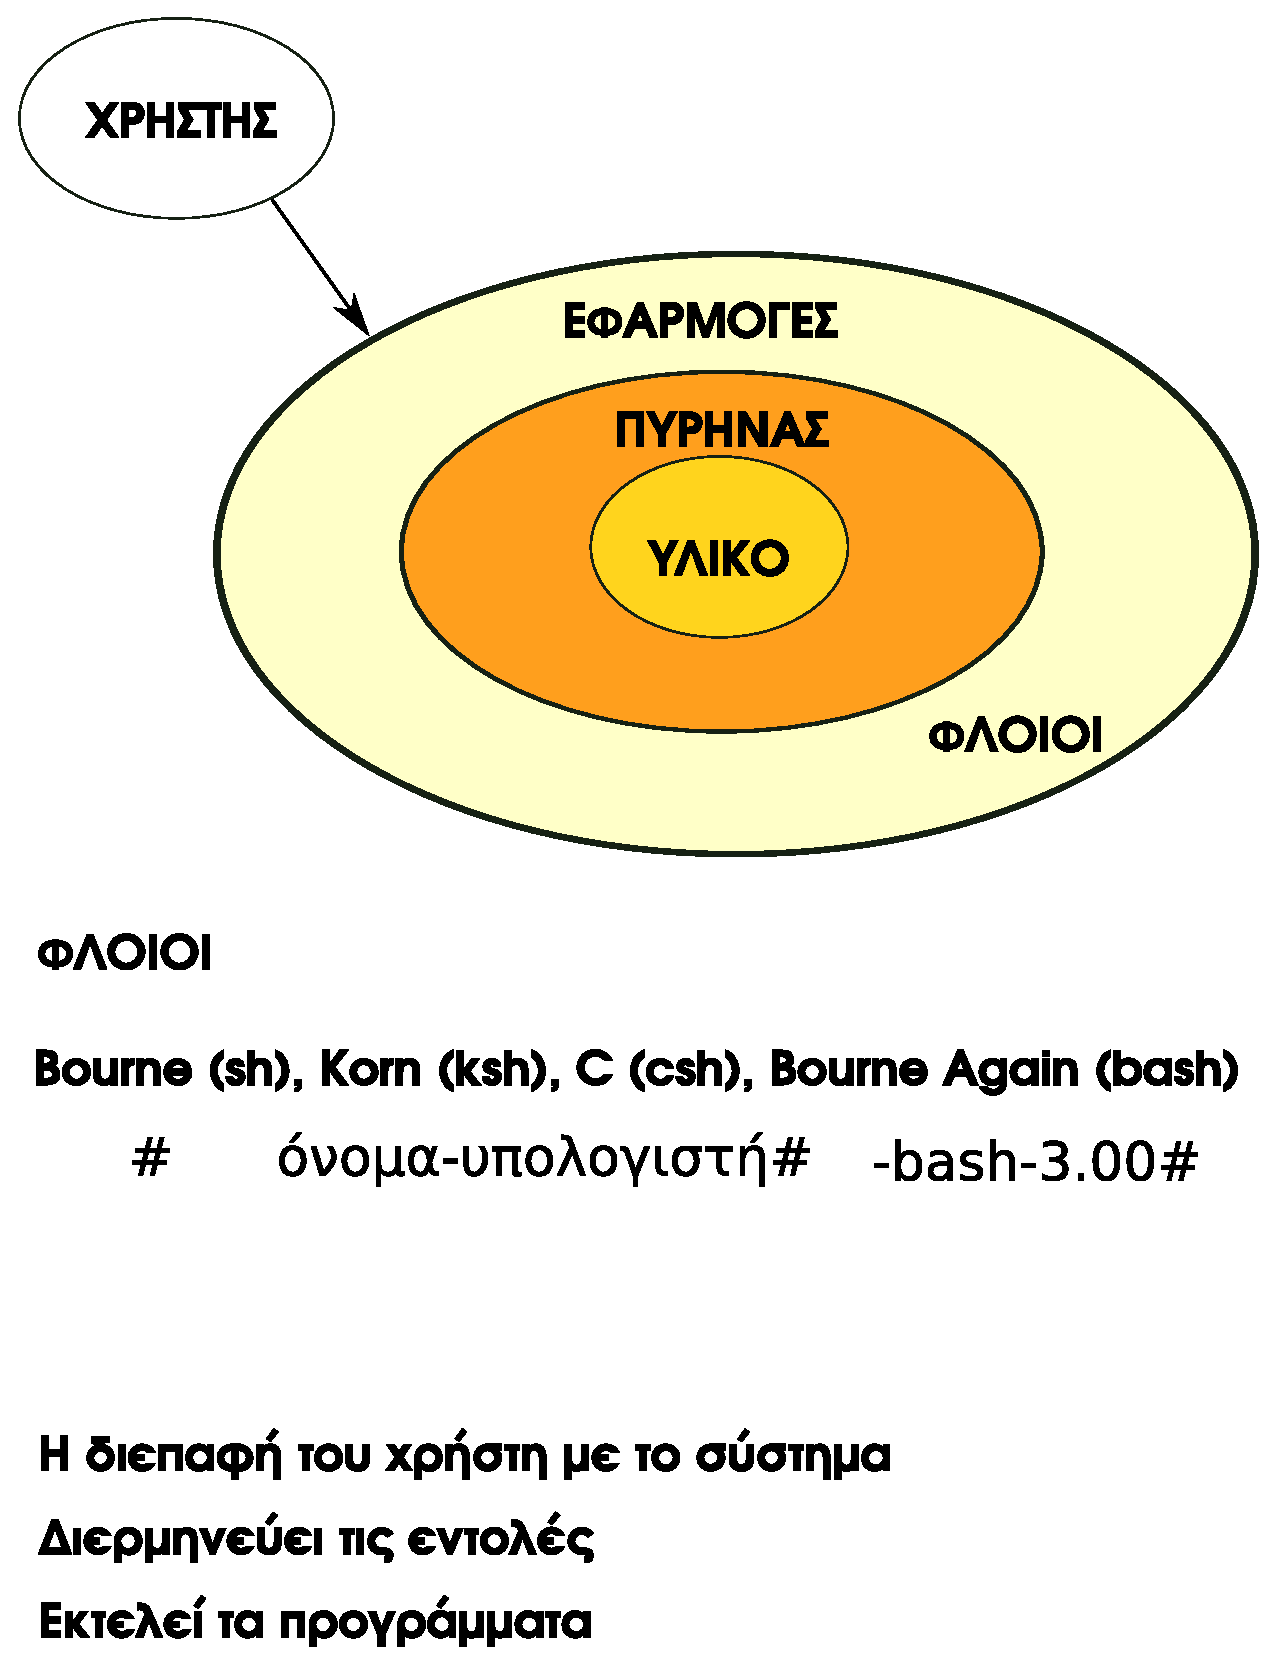
\includegraphics{shells.eps}}
  \scalebox{0.5}{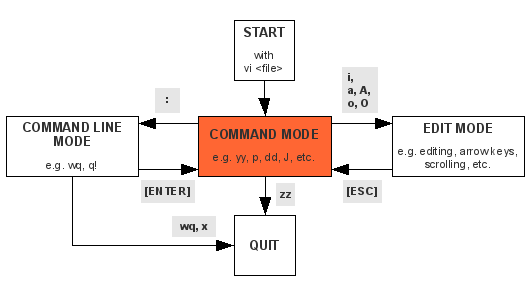
\includegraphics[angle=0]{images/vi_scheme.png}}
  \caption{Ο vi συνοπτικά}
\end{figure*} 

\begin{figure*}[!h]
	\centering
	%\scalebox{0.2}{\includegraphics{unix-tree.eps}}
	%\resizebox{\linewidth}{!}{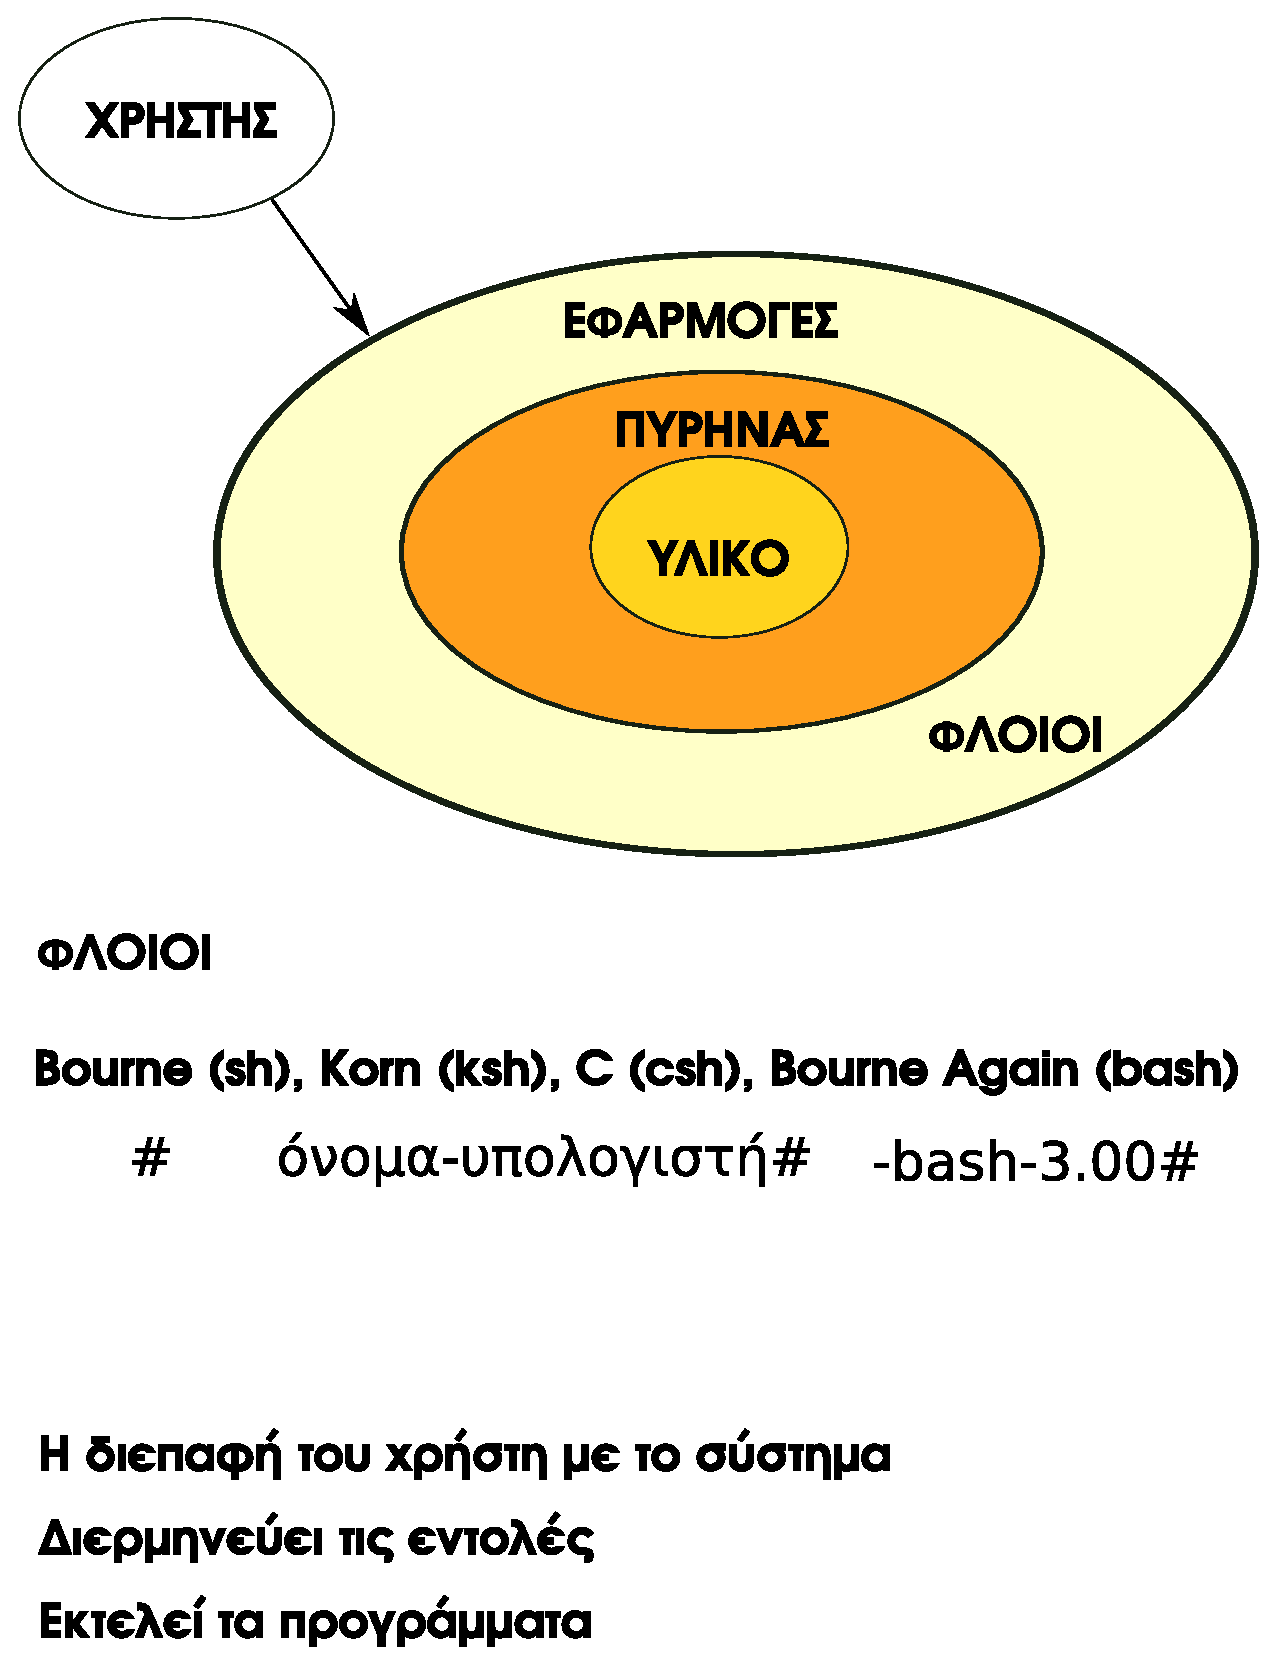
\includegraphics{shells.eps}}
	\scalebox{0.7}{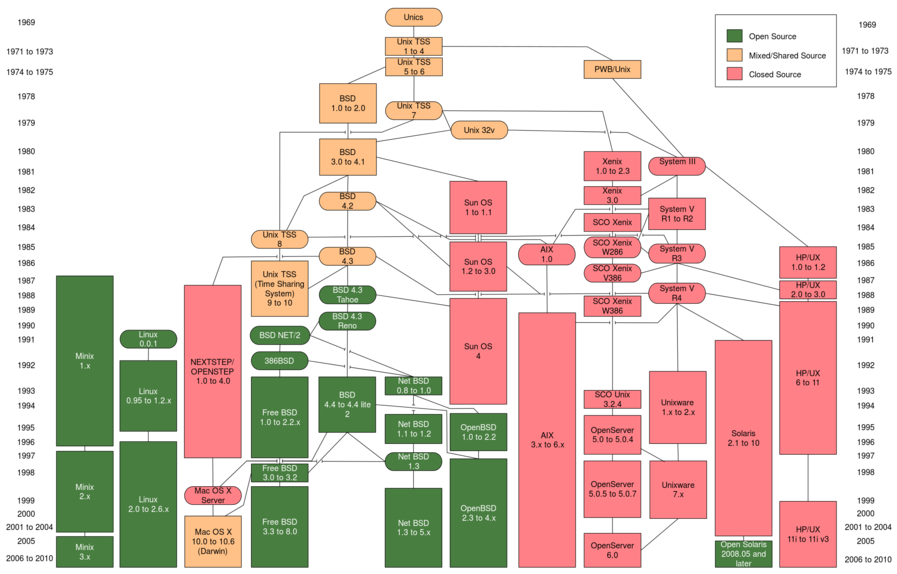
\includegraphics[angle=0]{images/unix_history.png}}
	\caption{Η ιστορία του UNIX}
\end{figure*}




